\documentclass{article}

\usepackage[margin=1in]{geometry}
\usepackage{amsmath,amsthm,amssymb}
\usepackage{bbm,enumerate,mathtools,mathrsfs}
\usepackage[hidelinks]{hyperref}
\usepackage{tikz}
\usetikzlibrary{matrix, arrows, patterns}

\newenvironment{problem}[2][Problem]{\begin{trivlist}
\item[\hskip \labelsep {\bfseries #1}\hskip \labelsep {\bfseries #2.}]}{\end{trivlist}}
\newenvironment{solution}[1][Solution.]{\begin{trivlist}
\item[\hskip \labelsep {\bfseries #1}]}{\end{trivlist}}
\newenvironment{problempart}[1]{\begin{trivlist}\item[\textbf{Part #1.}]}{\end{trivlist}}

\newenvironment{definition}[1][Definition.]{
  \begin{trivlist} \item[\hskip \labelsep {\bfseries #1}]
}{\end{trivlist}}

\newenvironment{example}[1][Example.]{
  \begin{trivlist} \item[\hskip \labelsep {\bfseries #1}]
}{\end{trivlist}}

\newenvironment{note}[1][Note.]{
  \begin{trivlist} \item[\hskip \labelsep {\bfseries #1}]
}{\end{trivlist}}

\newenvironment{theorem}[1][Theorem.]{
  \begin{trivlist} \item[\hskip \labelsep {\bfseries #1}]
}{\end{trivlist}}

\newenvironment{exercise}[1][Exercise.]{
  \begin{trivlist} \item[\hskip \labelsep {\bfseries #1}]
}{\end{trivlist}}

\newcommand{\set}[1]{\{ #1 \}}
\newcommand{\inv}[1]{#1^{-1}}
\newcommand{\ang}[1]{\langle #1 \rangle}
\newcommand{\paren}[1]{\left( #1 \right)}
\newcommand{\fn}[3]{#1 \colon #2 \rightarrow #3}
\newcommand{\wt}{\operatorname{wt}}
\newcommand{\id}{\operatorname{id}}

\begin{document}

\title{Math 533: Homework 6}
\author{Peter Kagey}
\date{April 10, 2019}

\maketitle

% -----------------------------------------------------
% First problem
% -----------------------------------------------------
\begin{problem}{1}
\end{problem}

\begin{proof} ~
  \begin{enumerate}[(a)]
    \item Let $\varphi$ send $\lambda \in \operatorname{Comp}(n)$ to its partial
    sums, but leaving off $n$. Then $\inv\varphi$ is just adding $n$ to the set and
    taking first differences. For example: \begin{align*}
      (4)          &\mapsto \set{}      \\
      (1, 3)       &\mapsto \set{1}     \\
      (2, 2)       &\mapsto \set{2}     \\
      (1, 1, 2)    &\mapsto \set{1,2}   \\
      (3, 1)       &\mapsto \set{3}     \\
      (1, 2, 1)    &\mapsto \set{1,3}   \\
      (2, 1, 1)    &\mapsto \set{2,3}   \\
      (1, 1, 1, 1) &\mapsto \set{1,2,3}.
    \end{align*}
    The refinement condition says that $\lambda = (\lambda_1, \lambda_2, \hdots, \lambda_n) \preceq (\lambda'_{1,1}, \hdots \lambda'_{1,k_1},\hdots, \lambda'_{n,1}, \hdots, \lambda'_{n,k_n}) = \lambda'$
    where $\lambda'_{i,1} + \hdots + \lambda'_{i,k_i} = \lambda_i$ for each $i$.
    Then it is clear that
    \begin{align*}
      \phi(\lambda)
        &= \set{\lambda_1, \lambda_1 + \lambda_2, \hdots, \lambda_1 + \hdots + \lambda_{n-1}} \\
        &\subseteq \set{
          \lambda'_{1,1},
          \hdots,
          \underbrace{\lambda'_{1,1} + \hdots + \lambda'_{1,k_1}}_{\lambda_1},
          \hdots,
          \underbrace{\lambda'_{1,1} + \hdots + \lambda'_{n-1,k_{n-1}}}_{\lambda_1 + \hdots + \lambda_{n-1}},
          \hdots,
          \lambda'_{1,1} + \hdots + \lambda'_{n,k_n-1}
        }.
    \end{align*}
    \item Gessel's fundamental basis is defined as \[
      F_\alpha
      = \sum_{\beta \preceq \alpha} M_\beta
      = \sum_{\beta \preceq \alpha} \sum_{i_1 < \cdots < i_k} x_{i_1}^{\beta_1} \cdots x_{i_k}^{\beta_k}
    \] so it follows by the refinement condition \begin{align*}
      F_\alpha
      &= \sum_{\varphi(\beta) \supseteq \varphi(\alpha)} \sum_{i_1 < \cdots < i_k} x_{i_1}^{\beta_1} \cdots x_{i_k}^{\beta_k}\\
      &= \sum_{\varphi(\beta) \supseteq \varphi(\alpha)} \sum_{\substack{
        i_{1,1} = \cdots = i_{1,m_1} <\\
        i_{2,1} = \cdots = i_{2,m_2} <\\
        \cdots  \\
        i_{k,1} = \cdots = i_{k,m_k}}} x_{i_{1,1}} \cdots x_{i_{1,n_1}} x_{i_{2,1}} \cdots x_{i_{k, n_k}} \\
      &= \sum_{\substack{
        i_1 \leq \hdots i_k\\
        i_j < i_{j+1} \text{ if } j \in \varphi(\alpha)
      }} x_{i_1} \hdots x_{i_k}.
    \end{align*}
    \item Let $f$ be a symmetric function written in the Schur basis. We'll
    check $\rho$ and $\psi$ on $s_\lambda$ and extend by linearity.
    For example $\lambda = (2,1,1)$ has SYT corresponding to the compositions
    $(2,1,1), (1,2,1),$ and $(1,1,2)$, which we'll index by the sets
    $\{2,3\}, \{1,3\},$ and $\{1,2\}$ respectively.
    \begin{align*}
      s_{(2,1,1)}       &= f_{(2,1,1)} + f_{(1,2,1)} + f_{(1,1,2)} \\
                        &= f_{\{2,3\}} + f_{\{1,3\}} + f_{\{1,2\}} \\
      \rho(s_{(2,1,1)}) &= \rho(f_{(2,1,1)}) + \rho(f_{(1,2,1)}) + \rho(f_{(1,1,2)}) \\
                        &= f_{(1,1,2)} + f_{(1,2,1)} + f_{(2,1,1)} \\
                        &= s_{(2,1,1)} \\
      \psi(s_{(2,1,1)}) &= \psi(f_{(2,1,1)}) + \psi(f_{(1,2,1)}) + \psi(f_{(1,1,2)}) \\
                        &= f_{\varphi(\{2,3\}^c)} + f_{\varphi(\{1,3\}^c)} + f_{\varphi(\{1,2\}^c)} \\
                        &= f_{\varphi(\{1\})} + f_{\varphi(\{2\})} + f_{\varphi(\{3\})} \\
                        &= f_{(1,3)} + f_{(2,2)} + f_{(3,1)} \\
      w(s_{(2,1,1)})    &= s_{(2,1,1)'} \\
                        &= s_{(3,1)} \\
                        &= f_{(1,3)} + f_{(2,2)} + f_{(3,1)}
    \end{align*}
    So in this particular example, $\rho$ is the identity and $\psi$ agrees with $w$.
    This is because under conjugation, inversions become non-inversions and vice versa,
    as illustrated here:
    \[
      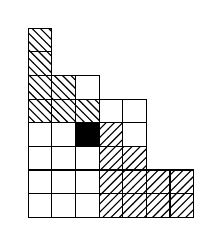
\begin{tikzpicture}[scale=0.3]
        \draw
          (0,0) grid (5,5)
          (0,5) grid (1,8)
          (1,5) grid (3,6)
          (5,0) grid (7,2)
        ;
        \fill[black] (2,3) rectangle (3,4);
        \draw[fill=blue, pattern=north west lines] (3,4)--(3,5)--(2,5)--(2,6)--(1,6)--(1,8)--(0,8)--(0,4)--cycle;
        \fill[fill=blue, pattern=north east lines] (3,4)--(4,4)--(4,3)--(5,3)--(5,2)--(7,2)--(7,0)--(3,0)--cycle;
      \end{tikzpicture}
    \]
    If the black box is filled with $i$, the upper section consists of possible
    positions for $i+1$ which create inversions, the lower section for non-inversions.
    These places switch under conjugation. (And conjugation sends SYT to SYT.)
  \end{enumerate}
\end{proof}
\pagebreak

% -----------------------------------------------------
% Second problem
% -----------------------------------------------------
\begin{problem}{2}
\end{problem}

\begin{proof} ~
  \begin{enumerate}[(a)]
    \item The eight classes of standard shifted tableau are: \\~\\
    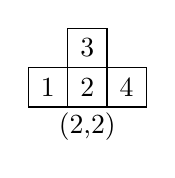
\begin{tikzpicture}[scale=0.5]
      \draw (-0.5,-0.5) rectangle (2.5,0.5) (0.5,-0.5)--(0.5,1.5)--(1.5,1.5)--(1.5,-0.5);
      \draw              (1,1) node {$3$}
        (0,0) node {$1$} (1,0) node {$2$} (2,0) node {$4$};
      \draw (1,-1) node {(2,2)};
    \end{tikzpicture}
    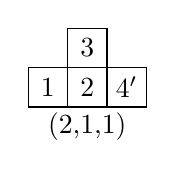
\begin{tikzpicture}[scale=0.5]
      \draw (-0.5,-0.5) rectangle (2.5,0.5) (0.5,-0.5)--(0.5,1.5)--(1.5,1.5)--(1.5,-0.5);
      \draw              (1,1) node {$3$}
        (0,0) node {$1$} (1,0) node {$2$} (2,0) node {$4'$}
      ;
      \draw (1,-1) node {(2,1,1)};
    \end{tikzpicture}
    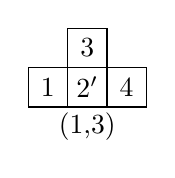
\begin{tikzpicture}[scale=0.5]
      \draw (-0.5,-0.5) rectangle (2.5,0.5) (0.5,-0.5)--(0.5,1.5)--(1.5,1.5)--(1.5,-0.5);
      \draw              (1,1) node {$3$}
        (0,0) node {$1$} (1,0) node {$2'$} (2,0) node {$4$}
      ;
      \draw (1,-1) node {(1,3)};
    \end{tikzpicture}
    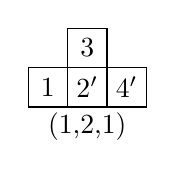
\begin{tikzpicture}[scale=0.5]
      \draw (-0.5,-0.5) rectangle (2.5,0.5) (0.5,-0.5)--(0.5,1.5)--(1.5,1.5)--(1.5,-0.5);
      \draw              (1,1) node {$3$}
        (0,0) node {$1$} (1,0) node {$2'$} (2,0) node {$4'$}
      ;
      \draw (1,-1) node {(1,2,1)};
    \end{tikzpicture}
    \\~\\
    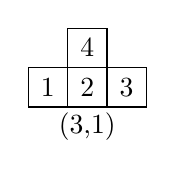
\begin{tikzpicture}[scale=0.5]
      \draw (-0.5,-0.5) rectangle (2.5,0.5) (0.5,-0.5)--(0.5,1.5)--(1.5,1.5)--(1.5,-0.5);
      \draw              (1,1) node {$4$}
        (0,0) node {$1$} (1,0) node {$2$} (2,0) node {$3$}
      ;
      \draw (1,-1) node {(3,1)};
    \end{tikzpicture}
    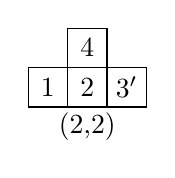
\begin{tikzpicture}[scale=0.5]
      \draw (-0.5,-0.5) rectangle (2.5,0.5) (0.5,-0.5)--(0.5,1.5)--(1.5,1.5)--(1.5,-0.5);
      \draw              (1,1) node {$4$}
        (0,0) node {$1$} (1,0) node {$2$} (2,0) node {$3'$}
      ;
      \draw (1,-1) node {(2,2)};
    \end{tikzpicture}
    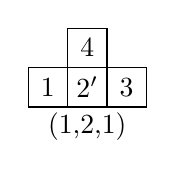
\begin{tikzpicture}[scale=0.5]
      \draw (-0.5,-0.5) rectangle (2.5,0.5) (0.5,-0.5)--(0.5,1.5)--(1.5,1.5)--(1.5,-0.5);
      \draw              (1,1) node {$4$}
        (0,0) node {$1$} (1,0) node {$2'$} (2,0) node {$3$}
      ;
      \draw (1,-1) node {(1,2,1)};
    \end{tikzpicture}
    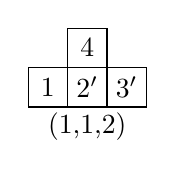
\begin{tikzpicture}[scale=0.5]
      \draw (-0.5,-0.5) rectangle (2.5,0.5) (0.5,-0.5)--(0.5,1.5)--(1.5,1.5)--(1.5,-0.5);
      \draw              (1,1) node {$4$}
        (0,0) node {$1$} (1,0) node {$2'$} (2,0) node {$3'$}
      ;
      \draw (1,-1) node {(1,1,2)};
    \end{tikzpicture}
    \\
    And each shows up with multiplicity four since we can prime the diagonals independently.
    \item It is clear from the example that $Q_\gamma$ is the sum over the
    standard shifted tableau of shape $\gamma$, and the multiplicity comes from
    the independence of priming the $\ell(\gamma)$ entries on the diagonal.
    \item Problem 1(c) worked out that \begin{align*}
      s_{(2,1,1)}       &= f_{(2,1,1)} + f_{(1,2,1)} + f_{(1,1,2)} \\
      s_{(3,1)}         &= f_{(1,3)} + f_{(2,2)} + f_{(3,1)}.
    \end{align*}
    Also, there are two standard young tableaux of shape $(2,2)$:
    \[
      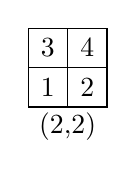
\begin{tikzpicture}[scale=0.5]
        \draw (-0.5,-0.5) rectangle (1.5,1.5) (-0.5,0.5)--(1.5,0.5) (0.5,-0.5)--(0.5,1.5) ;
        \draw (0,1) node {$3$} (1,1) node {$4$}
              (0,0) node {$1$} (1,0) node {$2$}
        ;
        \draw (0.5,-1) node {(2,2)};
      \end{tikzpicture}
      \hspace{5pt}
      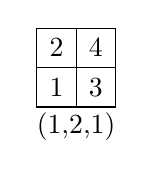
\begin{tikzpicture}[scale=0.5]
        \draw (-0.5,-0.5) rectangle (1.5,1.5) (-0.5,0.5)--(1.5,0.5) (0.5,-0.5)--(0.5,1.5) ;
        \draw (0,1) node {$2$} (1,1) node {$4$}
              (0,0) node {$1$} (1,0) node {$3$}
        ;
        \draw (0.5,-1) node {(1,2,1)};
      \end{tikzpicture}
    \] with corresponding expansion in Gessel's fundamental basis \[
      s_{(2,2)} = f_{(2,2)} + f_{(1,2,1)}.
    \]
    Thus \[
      Q_{(3,1)} = 4(s_{(2,1,1)} + s_{(3,1)} + s_{(2,2)}).
    \]
  \end{enumerate}
\end{proof}

\pagebreak
% -----------------------------------------------------
% Third problem
% -----------------------------------------------------
\begin{problem}{4}
\end{problem}

\begin{proof} ~
  \begin{enumerate}[(a)]
    \item If $\kappa\colon V \rightarrow \mathbb N_{>0}$ is proper, then acting
      on $\kappa$ by any permutation of the integers $\sigma$ also gives a proper
      coloring. This means that the sum is closed under permuting the indices,
      so $X_G$ is symmetric.
    \item By definition, the chromatic number of $G$ is \[
      \chi_G(n) = \#\set{\fn \kappa V {[n]} : \kappa \text{ is a proper coloring}}.
    \] This is identically \begin{align*}
      X_G(\underbrace{1, 1, \hdots, 1}_n, 0, 0, \hdots)
      &= \sum_{\substack{
        \kappa \text{ proper} \\
        \kappa(v) \leq n
      }} x_{\kappa(v_1)} \hdots x_{\kappa(v_n)}  \\
      &= \#\set{\fn \kappa V {[n]} : \kappa \text{ is a proper coloring}},
    \end{align*} as desired.
  \end{enumerate}
\end{proof}
\end{document}
